\documentclass[tikz,border=20pt]{standalone}
\usepackage{amsmath, amssymb}
\usetikzlibrary{positioning, arrows.meta, calc}

\begin{document}
	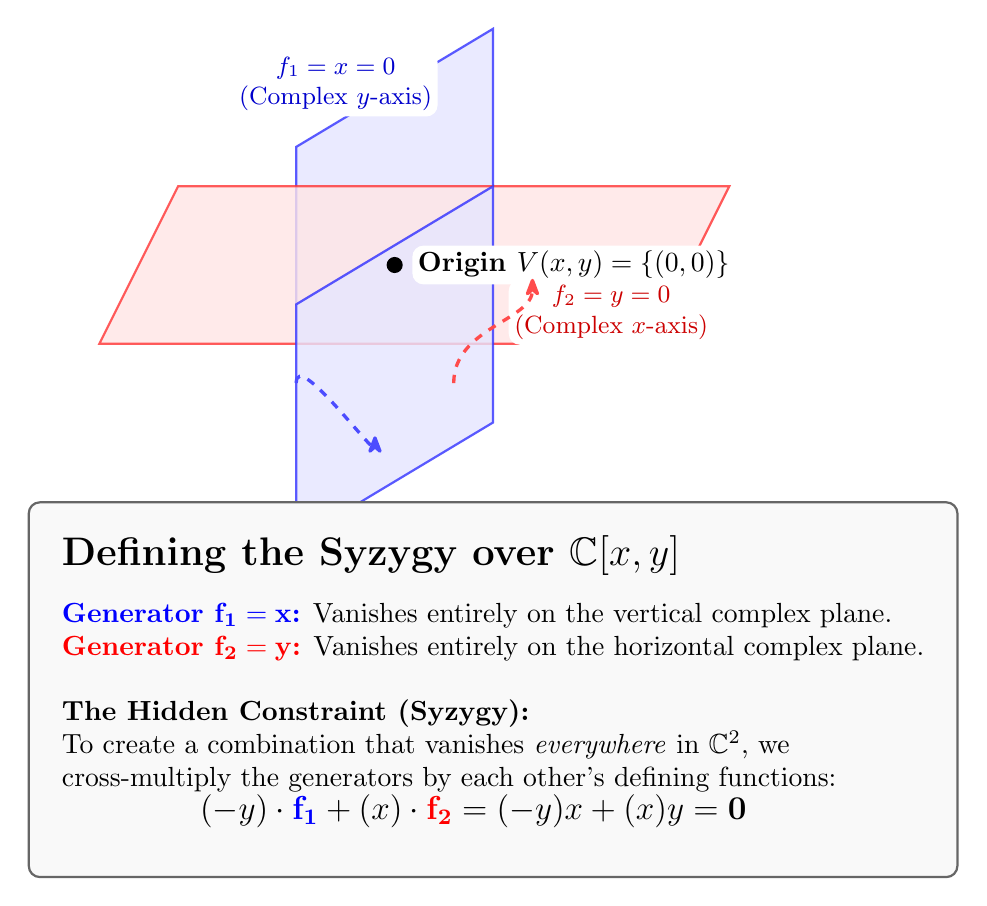
\begin{tikzpicture}[
		>={Stealth[round]}, thick,
		plane1/.style={fill=red!10, draw=red!80, opacity=0.8, thick},
		plane2/.style={fill=blue!10, draw=blue!80, opacity=0.8, thick},
		annotation/.style={font=\small, align=center, fill=white, inner sep=2pt, rounded corners}
		]
		
		% --- 3D coordinates for Plane 2 (V(x) - the Complex y-axis) ---
		% Drawn as a vertical-ish plane
		\coordinate (v1) at (-1, -3);
		\coordinate (v2) at (1.5, -1.5);
		\coordinate (v3) at (1.5, 3.5);
		\coordinate (v4) at (-1, 2);
		
		% --- 3D coordinates for Plane 1 (V(y) - the Complex x-axis) ---
		% Drawn as a horizontal-ish plane
		\coordinate (h1) at (-3.5, -0.5);
		\coordinate (h2) at (3.5, -0.5);
		\coordinate (h3) at (4.5, 1.5);
		\coordinate (h4) at (-2.5, 1.5);
		
		% Draw back half of Plane 2 (behind Plane 1)
		\filldraw[plane2] (v4) -- (v3) -- ($(v3)!0.4!(v2)$) -- ($(v4)!0.4!(v1)$) -- cycle;
		
		% Draw Plane 1
		\filldraw[plane1] (h1) -- (h2) -- (h3) -- (h4) -- cycle;
		
		% Draw front half of Plane 2 (in front of Plane 1)
		\filldraw[plane2] ($(v4)!0.4!(v1)$) -- ($(v3)!0.4!(v2)$) -- (v2) -- (v1) -- cycle;
		
		% The Intersection Point (The Origin)
		\coordinate (origin) at (0.25, 0.5);
		\filldraw[black] (origin) circle (2.5pt) 
		node[right=6pt, annotation, font=\bfseries] {Origin $V(x,y) = \{(0,0)\}$};
		
		% Labels for the geometric planes
		\node[annotation, text=blue!80!black] at (-0.5, 2.8) {$f_1 = x = 0$ \\ (Complex $y$-axis)};
		\node[annotation, text=red!80!black] at (3, -0.1) {$f_2 = y = 0$ \\ (Complex $x$-axis)};
		
		% --- Connection to Algebra ---
		\node[draw=black!60, fill=gray!5, rounded corners, inner sep=12pt, align=left, below=2cm of h1, xshift=5cm] (box) {
			\Large \textbf{Defining the Syzygy over $\mathbb{C}[x,y]$} \\[0.3cm]
			\normalsize \textcolor{blue}{\textbf{Generator $\mathbf{f_1 = x}$:}} Vanishes entirely on the vertical complex plane.\\
			\normalsize \textcolor{red}{\textbf{Generator $\mathbf{f_2 = y}$:}} Vanishes entirely on the horizontal complex plane.\\[0.4cm]
			\normalsize \textbf{The Hidden Constraint (Syzygy):} \\
			\normalsize To create a combination that vanishes \textit{everywhere} in $\mathbb{C}^2$, we \\
			\normalsize cross-multiply the generators by each other's defining functions:\\
			\vspace{0.2cm}
			\large \hspace*{1.5cm} $(-y) \cdot \textcolor{blue}{\mathbf{f_1}} + (x) \cdot \textcolor{red}{\mathbf{f_2}} = (-y)x + (x)y = \mathbf{0}$
		};
		
		% Pointers from the explanation to the geometry
		\draw[->, blue!70, dashed, very thick, shorten >= 5pt] 
		([yshift=1.5cm, xshift=-2.5cm]box.north) to[out=90, in=270] (0, -1.5);
		
		\draw[->, red!70, dashed, very thick, shorten >= 5pt] 
		([yshift=1.5cm, xshift=-0.5cm]box.north) to[out=90, in=270] (2, 0.5);
		
	\end{tikzpicture}
\end{document}